
\textbf{Avant de commencer}
Avant toute chose, créer un répertoire TP10 dans votre répertoire "Informatique". Sur le site \url{https://ptsilamartin.github.io/info/TP.html}, télécharger \lstinline{algorithmes_gloutons.py} que vous copiez dans votre répertoire TP10.\\

\emph{Rappel}: On prendra bien soin, dans tout le TP, de documenter les fonctions écrites et de les tester. Les tests seront présentés en commentaires dans le script.

\section*{Algorithme Glouton - Remplir un sac à dos}
\marginnote{A partir du travail de Nicolas VIDAL et de Nicolas COURRIER pour l'UPSTI.}

Un promeneur souhaite transporter dans son sac à dos le fruit de sa cueillette. La cueillette est belle, mais trop lourde pour être entièrement transportée dans le sac à dos. Des choix doivent être faits. Il faut que la masse totale des fruits choisis ne dépasse pas la capacité maximale du sac à dos.

Les fruits cueillis ont des valeurs différentes, et le promeneur souhaite que son chargement soit de la plus grande valeur possible.

\begin{figure}[h]
	\centering
		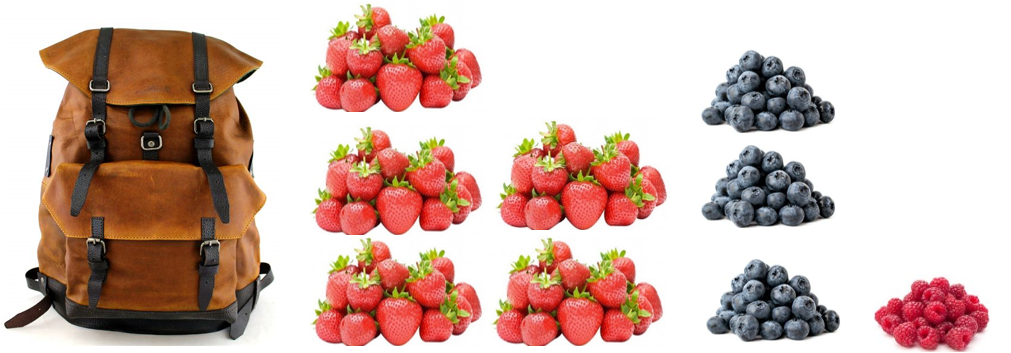
\includegraphics[width=.8\linewidth]{SacEtFruits.png}
	\label{fig:SacEtFruits}
\end{figure}



\begin{table}[h]
	\centering
		\begin{tabular}{|l|c|c|}
\hline
Fruits cueillis	& Prix au kilo & Quantité ramassée\\
\hline
framboises& 24 €/kg  & 1 kg \\
myrtilles & 16 €/kg & 3 kg  \\
fraises & 6 €/kg & 5 kg \\
mures & 3 €/kg & 2 kg \\
\hline
		\end{tabular}
	%	\caption{}
	\label{tab_fruit}
\end{table}

La capacité du sac à dos n’est que de 5 kg.

On suppose que la masse d’un unique fruit est négligeable par rapport à la masse totale du sac en charge.

\subsection*{Présentation de l’algorithme et implémentation}
\label{sec:PrésentationDeLAlgorithmeEtImplémentation}

Le principe pour optimiser le chargement est de commencer par mettre dans le sac la quantité maximale de fruits les plus chers par unité de masse. S'il y a encore de la place dans le sac, on continue avec les fruits les plus chers par unité de masse parmi ceux restants, … et ainsi de suite jusqu'à ce que le sac soit plein.\\
Il est possible qu'on ne puisse prendre qu'une fraction de la quantité de fruits disponible, si la capacité maximale du sac est atteinte. L'algorithme sera donc constitué d'une structure itérative, incluant une structure alternative.\\

Dans \lstinline{algorithmes_gloutons.py}, nous avons ébauché l'algorithme de résolution du problème et implémenté \lstinline{cueillette} par la liste des fruits \textbf{triée} par prix au kilo décroissant.\\
Un fruit est représenté par une liste \lstinline{fruit=[prix au kilo,nom,quantité ramassée]}.

\lstinline{cueillette = [[24,"framboises",1], [16,"myrtilles",3], [6,"fraises",5], [3,"mures",2]]}.

\begin{question}
Dans \lstinline{algorithmes_gloutons.py}, compléter la fonction \lstinline{sac_a_dos(L:list, capacite:int)} qui prend en argument une liste de listes \lstinline{L} modélisant la cueillette et la capacité du sac à dos, et appliquant la méthode décrite précédemment. Cette fonction renvoie :
\begin{itemize}
\item une liste de listes des fruits contenus dans le sac à dos avec leur masse correspondante de façon à avoir le chargement de valeur maximale ;
\item la valeur du chargement.
\end{itemize}
\end{question}

La liste \lstinline{cueillette} ne doit pas être modifiée. Vous pourrez si nécessaire utiliser une copie de la liste  \lstinline{cueillette} que vous pourrez modifier. La copie de liste de listes se fait avec les instructions :

\begin{lstlisting}
import copy # au début de votre script
L=copy.deepcopy(votreListe) # quand cela est nécessaire
\end{lstlisting}

\begin{question}
A la suite du script \lstinline{algorithmes_gloutons.py}, taper les lignes de code permettant d’utiliser la fonction \lstinline{sac_a_dos()} pour afficher les  fruits et les quantités à choisir pour remplir le sac à dos, à partir de la liste \lstinline{cueillette}. Exécuter votre programme et vérifier le résultat.
\end{question}


\vspace*{0.5cm}
Une variante de ce problème ne trouve pas de solution optimale par la méthode gloutonne. Nous l'étudions ci-après.

\subsection*{Version non fractionnaire du problème du sac à dos}
\label{sec:VersionNonFractionnaireDuProblèmeDuSacÀDos}

On suppose maintenant que les éléments à transporter ne sont pas fractionnables. Les fruits parmi lesquels choisir sont présentés dans le tableau suivant.


\begin{table}[h]
	\centering
		\begin{tabular}{|l|c|c|c|}
\hline
Fruits  & Prix au kilo & Masse d’un fruit & Quantité disponible\\
\hline
melon de cavaillon & 3 €/kg & 1 kg & 1\\
melon jaune  & 2.5 €/kg & 2 kg & 1\\
pastèque & 2 €/kg & 3 kg & 1 \\

\hline
		\end{tabular}
		%\caption{}
	\label{tab_fruit2}
\end{table}

Cet ensemble de fruits est modélisé dans \lstinline{algorithmes_gloutons.py} par :
\begin{itemize}
\item un fruit non fractionnable est représenté par une liste \lstinline{prix au kilo,nom,masse,quantité disponible}
\item une liste de listes \lstinline{fruitsDisponibles = [[3,"melon de cavaillon",1,1], [2.5,"melon jaune",2,1], [2,"pastèque",3,1]]}.
\end{itemize}



L’objectif est toujours de placer dans le sac à dos le chargement de valeur maximale, de masse totale inférieure à 5kg. Par contre, les éléments n’étant fractionnables, il est possible que les choix successifs mène à un chargement qui ne remplit pas complètement le sac à dos.

On se propose de tester la méthode gloutonne pour cette nouvelle formulation. 

 

\begin{question}
Dans \lstinline{algorithmes_gloutons.py}, copier-coller \lstinline{sac_a_dos(L, capacite)} que vous renommerez \lstinline{sac_a_dos_V2(L, capacite)} et adapter la fonction de sorte qu’elle applique la méthode gloutonne à la version non fractionnaire du problème. %Pour cela, il faut :
%\begin{itemize}
%	\item {commenter la structure conditionnelle permettant de continuer à remplir le sac si sa capacité restante est inférieure à la masse du i-ème fruit,}
%	\item {adapter la condition de la structure itérative de sorte à ne continuer à remplir le sac que si la capacité le permet.}
%\end{itemize}


\end{question}

\begin{question}
Le résultat obtenu est-il optimal ? Comparer avec la solution \lstinline{S = [2.5,"melon jaune",2,1], [2,"pastèque",3,1]]}. Quelle est la solution dont la valeur est maximale ?
\end{question}

\begin{question}
De la propriété du choix glouton et de la propriété de la sous-structure optimale, laquelle n’est pas respectée dans cette formulation du problème ? En quoi l’autre propriété l’est ?
\end{question}

 
%Cette version du problème du sac à dos n’est pas adaptée à la méthode gloutonne. %Le cours de deuxième année vous permettra d’aborder la programmation dynamique qui offre une solution optimale à ce problème : son principe consiste en l’étude de toutes les combinaisons possibles afin de ne retenir que la combinaison optimale.


\section*{Le problème du choix d'activité}
%\setcounter{cexo}{0}
\subsection*{Présentation du problème}

Le problème du choix d'activité (PCA) concerne le problème d'ordonnancement de plusieurs activités qui rivalisent pour l'utilisation exclusive d'une ressource commune.\\
Une application concrète est l'allocation d'une salle à différents conférenciers au cours d'une journée. Plusieurs personnes souhaitent effectuer une conférence, mais ces conférences ont lieu à des horaires définis imposés par la disponibilité de chaque conférencier.\\
 Certaines conférences démarrent alors que d'autres ne sont pas encore terminées. Il n'est donc pas possible d'attribuer la salle à chaque conférencier pour chacune de ses conférences, et il faut faire des choix.\\ 
La solution optimale est celle qui permettra au plus grand nombre de conférences de se tenir.


\begin{figure}[h]
	\centering
%		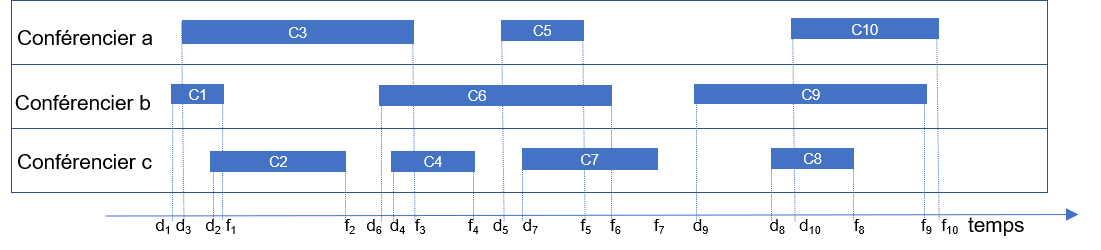
\includegraphics{image/conferences.png}
		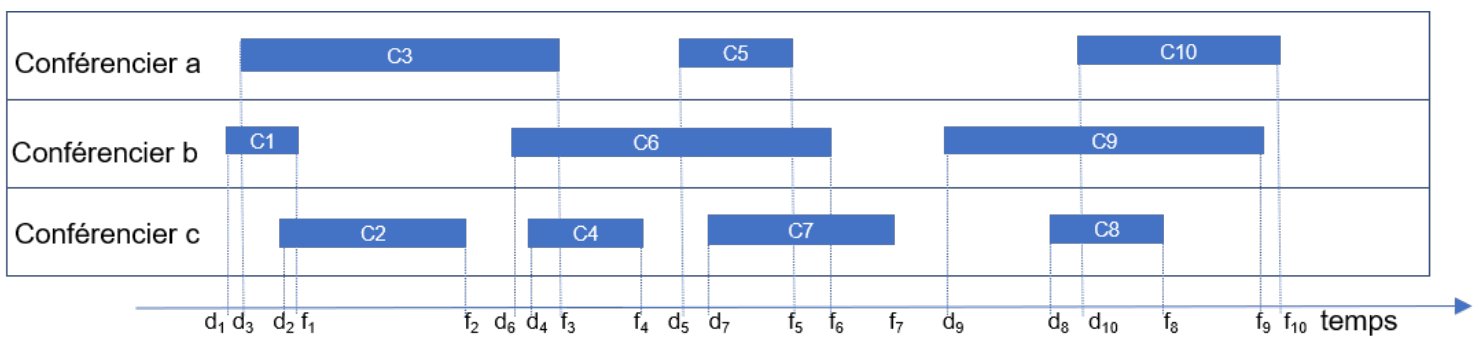
\includegraphics[width=\linewidth]{conf.png}
		\caption{Conférences parmi lesquelles choisir pour établir le planning de la salle de conférences}
	\label{fig:conf}
\end{figure}


Les conférences sont définies par leur heure de début et leur heure de fin. La conférence $c_i$ aura pour heure de début $d(c_i)$ et pour heure de fin $f(c_i)$.

Nous supposerons que les conférences ont été triées dans l'ordre croissant de leurs dates de fin. Si nous travaillons avec un ensemble C de n conférences, on a :
\begin{center} 
$f(c_1)<f(c_2)<\ldots<f(c_{n-1})<f(c_n)$
\end{center} 

On a bien affaire ici à un problème d'optimisation :
\begin{itemize}
\item soit $S={\{s_1,s_2,\ldots,s_k\}}$ l'ensemble des conférences constituant la solution ;
\item l'objectif : maximiser le nombre de conférences : maximiser $|S|$ ;
\item la contrainte :  les conférences doivent être compatibles, pour tout $i,j\in {\{1,…,k\}}$, on doit avoir $f(s_i )\leqslant d(s_j)$ ou $f(s_j )\leqslant d(s_j)$.
\end{itemize}

\subsection*{La solution gloutonne}

Dans notre application, le premier choix glouton consiste à choisir la conférence qui termine le plus tôt possible, préservant ainsi la disponibilité de la salle pour les conférences ultérieures.

Lorsqu'un choix de conférence a été fait, on procède de la même manière pour le choix suivant, mais il y a la contrainte de compatibilité : il faut choisir une conférence compatible avec celles qui ont déjà été choisies : On ne peut choisir qu'une conférence qui débute après la fin de la dernière conférence choisie. Si on note $C$ l'ensemble des conférences, et $S$ l'ensemble des conférences qui constituent notre solution optimale, à l'itération $k$ on a :
$S={s_1,s_2,\ldots,s_k}$ et $S\subset C$.

Alors il faut choisir la conférence $c_i \in C-S$ telle que $d(c_i )\leq f(s_k)$. 
L’algorithme construit alors un ensemble $S$ de conférences mutuellement compatibles, c’est-à-dire tel que :
$d(s_1 )<f(s_1 )\leq d(s_2)<f(s_2)\leq \ldots \leq d(s_j )<f(s_j)$.

\subsection*{Algorithme et test à la main }

\textbf{Paramètres : } $C$ est la liste des conférences, représentées par leurs dates de début et de fin, et leur intitulé \lstinline{[d(ci),f(ci),'ci']}.

\textbf{Résultat : } La liste \lstinline{Planning} de taille maximale de conférences compatibles.

\textbf{Algorithme : }
\begin{itemize}
\item la liste \lstinline{planning} est initialisée avec la première conférence ;
\item la variable \lstinline{fin} prend la valeur de la fin de la première conférence ;
\item pour tous les éléments $c_i$ de la liste \lstinline{C}, on teste si $c_i[0]$>=fin, alors on insère $c_i$ dans le planning et on remplace la valeur de \lstinline{fin} par $c_i[1]$, sinon, on ne fait rien.
\end{itemize}

%\begin{lstlisting}
%Planning <- [C[0]]   #les conférences étant classées par ordre croissant de leur heure de fin, 
%Fin <-  C[0][1]        #on sait que la première valeur de C correspond au premier choix glouton 
%Pour tous les elements c_i de la liste C :
%	Si c_i[0] >= Fin :
%		Inserer c_i a la suite de Planning
%		Fin <- c_i[1]
%\end{lstlisting}



\begin{question}
Exécuter à la main cette méthode en utilisant l'ensemble de conférences illustré sur la figure \ref{fig:conf}.
\end{question}

\subsection*{Implémentation}
\label{sec:Implémentation}

On modélise l'ensemble \lstinline{C} des conférences par une liste dont chaque élément modélise une conférence. Chaque conférence est modélisée par une liste de la date de début de type \lstinline{float} avec par exemple 8.45 qui correspond à 8h45, la date de fin de type \lstinline{float}, et l'intitulé de la conférence de type \lstinline{str}. Cette liste est ordonnée par ordre croissant de la date de fin des conférences. Ainsi, l'exemple représenté sur la figure \ref{fig:conf} pourrait être modélisé par la liste :

 

\lstinline{L=[[8,9,"C1"],[8.45,10.3,"C2"],[8.1,11.3,"C3"],[11.15,11.45,"C4"],[12,12.45,"C5"],[11,13,"C6"], [12.3,14,"C7"],[16,17,"C8"],[15,18,"C9"],[16.2,18.15,"C10"]]}


 

 

\begin{question}
\'Ecrire la fonction \lstinline{choix_conferences(C:list)->list} qui prend en argument une liste de conférences \lstinline{C}, et qui applique la méthode décrite précédemment. 
Le résultat est une liste de conférences mutuellement compatibles, de longueur maximale.
\end{question}

 


\begin{question}
\'Ecrire les instructions permettant d'utiliser la fonction \lstinline{choix_conferences(C:list)->list} pour déterminer la liste des conférences retenues parmi les conférences listées dans \lstinline{L}. Comparer le résultat avec celui obtenu avec le test à la main.
\end{question}

 

On observe que le résultat obtenu est bien un optimal. Cependant, il existe d'autres solutions, toutes autant optimales, par exemple C2, C4, C7, C10 ou encore C1, C4, C5, C9.

\subsection*{Le choix glouton et le sous problème optimal}
\label{sec:LeChoixGloutonEtLeSousProblèmeOptimal}
Un algorithme glouton ne mène pas forcément à une solution optimale d'un problème d'optimisation.
Pour qu'un algorithme glouton soit adapté à la résolution d'un problème, il faut que le problème ait la propriété de sous-structure optimale, c'est-à-dire que la solution optimale du problème contient des solutions optimales des sous-problèmes.

Une résolution par la méthode gloutonne nécessite par ailleurs que les choix gloutons successifs engendrent une solution optimale globalement. C’est la propriété de choix glouton.

Pour notre application :
$S={s_1,s_2,…,s_k}$  est le résultat de notre algorithme. On montre par récurrence que pour tout $j\leq k$, le sous-ensemble $S_j={s_1,s_2,… ,s_j}$ de S est un sous ensemble d’une solution optimale :
\begin{itemize}
	\item Pour j=0 : l'ensemble $S_j$ est un ensemble vide, et est donc un sous-ensemble d'une solution optimale,
	\item Pour j>0 : Soit T une solution optimale telle que pour $j<k$,  $S_j\subset T$  (T contient les activités $s_1,s_2,… ,s_j$). On note b l’élément suivant $s_j$ dans T: 
	\begin{itemize}
		\item On a $f(s_{j+1}  ) \leq f(b)$ (en raison du choix glouton, on choisit l’activité que finit le plus tôt),
		\item les éléments de T sont tous compatibles, ainsi chaque élément succédant à b débute après la fin de b et de $s_{j+1}$.
	\end{itemize}
Ainsi $T- \left\{b\right\} \bigcup \left\{s_{j+1} \right\}$ est une solution optimale, de même cardinal  que $S$, et elle contient $s_1,s_2,… ,s_{j+1} $
\end{itemize}
	
$S$ est donc une solution optimale.
On a bien démontré que l’algorithme du choix d’activité est correct, présente la propriété de sous-structure optimale, et que le choix glouton permet d’arriver à une solution optimale globalement.


\begin{question}
\'Ecrire la fonction \lstinline{choix_conferences_recursif(C:list,k:int,n:int)->list} qui prend en argument une liste de conférences \lstinline{C}, un indice \lstinline{k} et \lstinline{n} la taille de C, et qui applique la méthode décrite précédemment de manière récursive. 
Le résultat est une liste de conférences mutuellement compatibles, de longueur maximale.
\end{question}

\vfill


Références :
\begin{itemize}
\item Algorithmique – Cormen Leiserson Rivest Stein - Dunod 
\item Matroïdes et algorithmes gloutons : UNE INTRODUCTION - Pierre Béjian 
\item Algorithmes gloutons - Ressource éduscol NSI 
\item Algorithmes gloutons - Emmanuel Beffara - lis-lab 
\end{itemize}

